\documentclass[UTF8]{ctexart}
\usepackage{graphicx}
\title{实验三:流水线CPU}
\author{陈子轩 516030910545}
\date{\today}

\begin{document}
\maketitle
\section{实验目的和实验步骤}
请参考实验指导书
\section{实验设计思路}
\subsection{整体工程的构建}
本次流水线CPU大部分代码需要自己来写,但是总体架构是清晰的,如图一
\begin{figure}
    \centering
    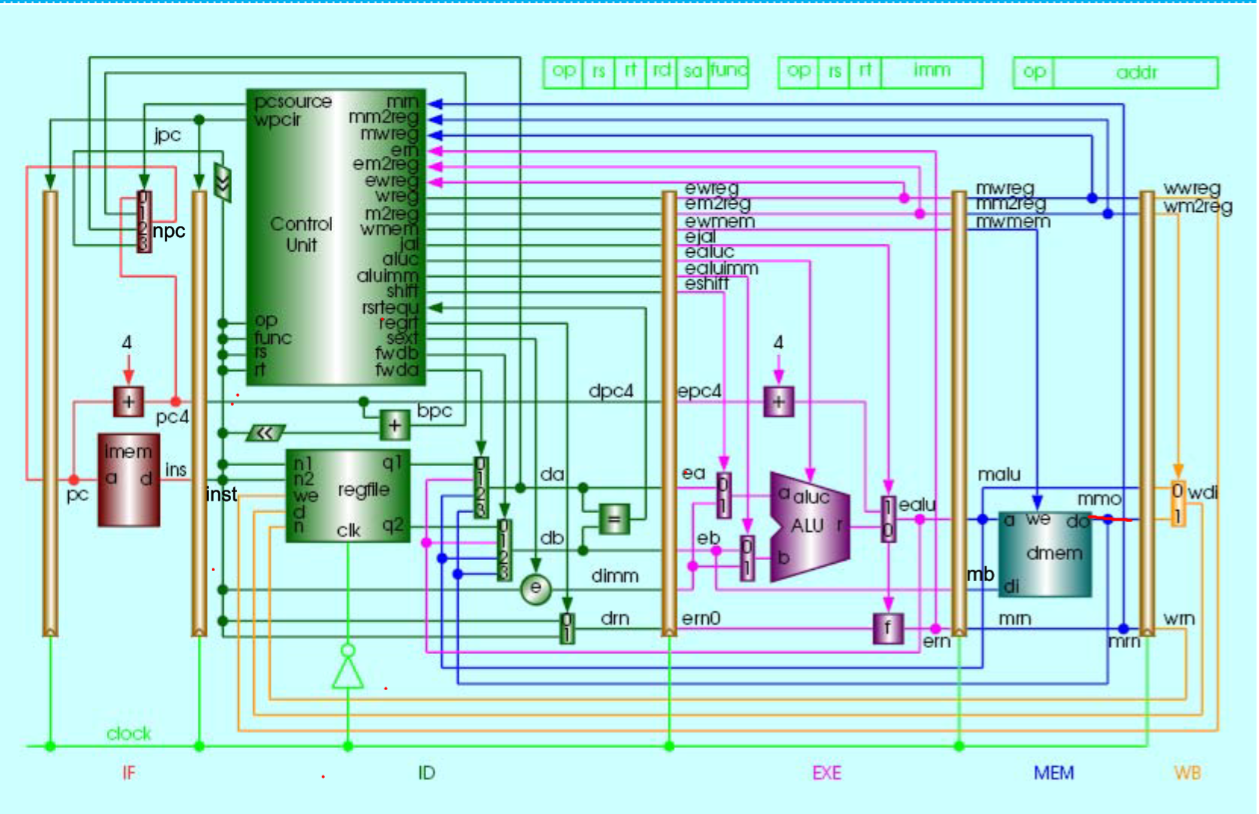
\includegraphics[width=1\textwidth]{pipelinecpu.png}
    \caption{流水线CPU整体架构}
\end{figure}
我的设计是将其分为4个中间流水线寄存器和五个流水段,流水段内大部分是组合逻辑,流水线寄存器内是时序逻辑。
\subsection{MEM阶段的构建}
在设计中我采用了3个in\_port接口对应操作数1(operand1, $sw[3:0]$),操作数2(operand2, $sw[7:4]$),和操作类型(type of operation, $sw[9:8]$)。采用了三个out\_port接口对应操作数1(operand1, hex0, hex1),操作数2(operand2, hex2, hex3)和操作结果(result, hex4, hex5)。实际采用了四种算术运算(add, sub, and, or)进行测试。

\subsection{FPGA适配器的构建}
上述情况中我们需要将各种in\_port和out\_port对应到我们的FPGA上。
\newline
\begin{tabular}{|l|l|} %l(left)居左显示 r(right)居右显示 c居中显示
	\hline
	in\_port0  & sw[3:0]    \\
	\hline
	in\_port1  & sw[7:4]    \\
	\hline
	in\_port2  & sw[9:8]    \\
	\hline
	out\_port0 & hex0, hex1 \\
	\hline
	out\_port1 & hex2, hex3 \\
	\hline
	out\_port2 & hex4, hex5 \\
	\hline
\end{tabular}

\section{源代码}
下面提供一些自己设计的代码,实验提供的源码则作忽略,寄存器代码形式单一,因此位简单起见只提供其中一个的代码
\begin{verbatim}
module 	pipeif(pcsource,pc,bpc,da,jpc,npc,pc4,ins,mem_clock); // IF stage

    //IF取指令模块,注意其中包含的指令同步ROM存储器的同步信号,
    //即输入给该模块的mem_clock 信号,模块内定义为 rom_clk。// 注意 mem_clock。
    //实验中可采用系统 clock 的反相信号作为mem_clock(亦即 rom_clock),
    //即留给信号半个节拍的传输时间。

    input [31:0] 	pc, bpc, da, jpc;
    input [1:0]		pcsource;
    input 			mem_clock;
    output [31:0] 	npc, ins, pc4;
    wire 	[31:0] 	pc4; //输入到pcmux的线

    assign pc4 = pc + 4;

    lpm_rom_irom irom (pc[7:2],mem_clock,ins);

    mux4x32 muxpc(pc4, bpc, da, jpc, pcsource, npc);

endmodule

module pipedereg ( dwreg,dm2reg,dwmem,daluc,daluimm,da,db,dimm,drn,
                dshift,djal,dpc4,clock,resetn,ewreg,em2reg,ewmem,
                ealuc,ealuimm,ea,eb,eimm,ern0,eshift,ejal,epc4 );

    input         dwreg,dm2reg,dwmem,djal,daluimm,dshift;
    input  [31:0] dpc4,da,db,dimm ;
    input  [3:0]  daluc;
    input  [4:0]  drn;
    wire          dwreg,dm2reg,dwmem,djal,daluimm,dshift;
    wire   [31:0] dpc4,da,db,dimm ;
    wire   [3:0]  daluc;
    wire   [4:0]  drn;

    input         clock,resetn;
    wire          clock,resetn;

    output        ewreg,em2reg,ewmem,ejal,ealuimm,eshift;
    output [31:0] epc4,ea,eb,eimm ;
    output [3:0]  ealuc;
    output [4:0]  ern0;

    reg           ewreg,em2reg,ewmem,ejal,ealuimm,eshift;
    reg    [31:0] epc4,ea,eb,eimm ;
    reg    [3:0]  ealuc;
    reg    [4:0]  ern0;

    always @ (negedge resetn or posedge clock)
        if (resetn == 0)
            begin
                epc4       <= 32'b0;
                ea         <= 32'b0;
                eb         <= 32'b0;
                eimm       <= 32'b0;
                ealuc      <=  4'b0;
                ern0       <=  5'b0;
                ewreg      <=  1'b0;
                em2reg     <=  1'b0;
                ewmem      <=  1'b0;
                ejal       <=  1'b0;
                ealuimm    <=  1'b0;
                eshift     <=  1'b0;
            end
        else
            begin
                epc4       <=  dpc4;
                ea         <=  da;
                eb         <=  db;
                eimm       <=  dimm;
                ealuc[3:0] <=  daluc[3:0];
                ern0       <=  drn;
                ewreg      <=  dwreg;
                em2reg     <=  dm2reg;
                ewmem      <=  dwmem;
                ejal       <=  djal;
                ealuimm    <=  daluimm;
                eshift     <=  dshift;
            end
endmodule

module pipeexe ( ealuc,ealuimm,ea,eb,eimm,eshift,ern0,epc4,ejal,ern,ealu);

    input   [3:0]  ealuc;
    input          ealuimm,eshift,ejal;
    input  [31:0]  ea,eb,eimm,epc4 ;       //esa
    input   [4:0]  ern0;

    output  [4:0]  ern;
    output [31:0]  ealu;

    wire   [31:0]  epc8,alu_ina,alu_inb,aluout;
    wire   [31:0]  sa;
    wire           zero;
    wire           eshift;


    assign  epc8 = epc4 + 8'h4;

    assign  sa[31:0] = { 27'b0,eimm[10:6] }; // extend sa to 32 bits for sll/srl/sra;

    // wire [31:0]   dsa = { 27'b0, inst[10:6] }; // extend to 32 bits from sa for shift instruction

    assign  ern[4:0] = ern0 | {5{ejal}}; // jal: r31 <-- p4;  // 31 or ern0/ reg_dest - mc
    //  muxff ernf (ern0,ejal,ern);  // zr


    mux2x32 mux_shift  (ea,sa,eshift,alu_ina);

    mux2x32 mux_aluimm (eb,eimm,ealuimm,alu_inb);

    alu al_unit (alu_ina,alu_inb,ealuc,aluout,zero );

    mux2x32 mux_jal (aluout,epc8,ejal,ealu);

endmodule

module pipemem ( mwmem,malu,datain,clock,mem_clk,mmo,
                sw, hex0, hex1, hex2, hex3, hex4, hex5);	// MEM stage

    //MEM数据存取模块。其中包含对数据同步RAM的读写访问。// 注意 mem_clock。
    //输入给该同步RAM的mem_clock 信号,模块内定义为 ram_clk。
    //实验中可采用系统 clock 的反相信号作为mem_clock 信号(亦即 ram_clk),
    //即留给信号半个节拍的传输时间,然后在mem_clock 上沿时,读输出、或写输入。

    input  			mwmem, clock, mem_clk;
    input [9:0]		sw;
    input [31:0]   malu, datain;

    output [6:0] 	hex0, hex1, hex2, hex3, hex4, hex5; //mb是sw写入的数据, mmo是读出的数据,malu是写入的地址
    output [31:0] 	mmo;


    wire [31:0]  	in_port0,in_port1, in_port2;

    reg [31:0] 		out_port0, out_port1, out_port2, io_dataout;
    wire [31:0] 	mem_dataout;
    wire write_enable, write_dmem_enable;

    assign write_enable = mwmem;

    assign write_dmem_enable = (malu[7] == 1) ? 1'b0 : write_enable;

    lpm_ram_dq_dram  dram(malu[6:2], mem_clk, datain, write_dmem_enable, mem_dataout);
    assign mmo = (malu[7] == 1)? io_dataout : mem_dataout;

    in_port_adapter FPGA2port(sw, in_port0, in_port1, in_port2);
    out_port_adapter port2FPGA(hex0, hex1, hex2, hex3, hex4, hex5, out_port0, out_port1, out_port2);

    always @(posedge mem_clk)
        begin
            if (malu[7:2] == 6'b100000) //128 对应操作数1
            io_dataout <= in_port0;
            else if (malu[7:2] == 6'b100001) //132 对应操作数2
            io_dataout <= in_port1;
            else if (malu[7:2] == 6'b100010) //136 对应操作类型
            io_dataout <= in_port2;
            else
            io_dataout <= 0;

            out_port0 <= in_port0;
            out_port1 <= in_port1;
            if(malu[7:2] == 6'b100011)
            out_port2 <= datain;
        end

endmodule

module in_port_adapter(sw, in_port0, in_port1, in_port2);

    input [9:0] sw;
    output [31:0] in_port0, in_port1, in_port2;

    assign in_port0 = {28'b0, sw[3:0]};
    assign in_port1 = {28'b0, sw[7:4]};
    assign in_port2 = {30'b0, sw[9:8]};

endmodule

module out_port_adapter(hex0, hex1, hex2, hex3, hex4, hex5, out_port0, out_port1, out_port2);

    input [31:0] out_port0, out_port1, out_port2;

    output [6:0] hex0, hex1, hex2, hex3, hex4, hex5;

    wire [3:0] a0, a1, b0, b1, c0, c1;
    assign a0 = out_port0 % 10;
    assign a1 = out_port0 / 10;
    assign b0 = out_port1 % 10;
    assign b1 = out_port1 / 10;
    assign c0 = out_port2 % 10;
    assign c1 = out_port2 / 10;

    sevenseg h0(a0, hex0);
    sevenseg h1(a1, hex1);
    sevenseg h2(b0, hex2);
    sevenseg h3(b1, hex3);
    sevenseg h4(c0, hex4);
    sevenseg h5(c1, hex5);

endmodule


//4bit 的BCD码至 7 段 LED数码管译码器模块
module sevenseg ( theta, ledsegments);
    input [3:0] theta;
    output [6:0] ledsegments;
    reg [6:0] ledsegments;
    always @ (*)
        case(theta)
            // //gfe_dcba 654_3210
            0: ledsegments = 7'b100_0000;				// DE2C板上的数码管为共阳极接法
            1: ledsegments = 7'b111_1001;
            2: ledsegments = 7'b010_0100;
            3: ledsegments = 7'b011_0000;
            4: ledsegments = 7'b001_1001;
            5: ledsegments = 7'b001_0010;
            6: ledsegments = 7'b000_0010;
            7: ledsegments = 7'b111_1000;
            8: ledsegments = 7'b000_0000;
            9: ledsegments = 7'b001_0000;
            default: ledsegments = 7'b111_1111; 	// 其它值时全灭
        endcase
endmodule


\end{verbatim}
\end{document}